\section{Problem Statement}

\acrfull{lfd} is defined as a technique that develops policy from examining
state to action mappings \cite{argall_survey_2009}. The state are expressed in
terms of the features and the actions are the motion primitives. The action
causes changes in the state of the world. The world consist of the robot and
the environment. 

The \acrshort{lfd} problem can be defined as follows \cite{argall_survey_2009}. 

The world consist of states $S$ and actions $A$. The mapping between states by
way of actions is defined by a probabilistic transition function $T(s`|s, a) $
; $S \times A \times S \rightarrow [0,1]$. $s`$ is the resultant state due to
the execution of the action $a$ on the initial state $s$. As we all know the
world is not fully observable all the time. Only a part of the world $Z$ is
observable. The learning has to be made on the observable states $Z$.

A policy $\pi : Z \rightarrow A $ selects action based on observations of world
state. A policy determines which action $a$ to execute from $A$ based on the
observations $Z$. 


The demonstrations used in our approach consist of pairs of initial state and
final state. Initial state is the state before the execution of an action while
final state is the state after the execution of the state. The demonstrations
$d$ consist of pairs of demonstrated initial state $z$ and final state $z`$
Demonstrations $d \in D$ formally as $k$ pairs of initial-final states: $d =
{(z^i , {z`}^i)} \text{where} (z^i, {z`}^i) \in Z \text{and}  i = 0,...,k$

\subsection{Deriving a policy: Goal based mapping}

In these methods of policy learning of \acrshort{lfd}, the policy tries to
predict the state of the world once the action is executed based on the current
state of the world.

The perspective adopted is that multiple demonstrations of the same action can
help to understand the key aspects of the action. In other words, when an
action shares similar goal across multiple demonstrations, it might suggest
that corresponding goal must be achieved in-order to reproduce the action. So
these methods of policy learning takes the demonstrations as input and provides
a list of goals to be satisfied as output for reproduction of the action.

This prediction is the passed to a planner who tries to find a plan to execute
the action to reach the predicted goal state as illustrated in figure \ref{goal
based learning}(\cite{argall_survey_2009})
\begin{figure}[htp]
\centering
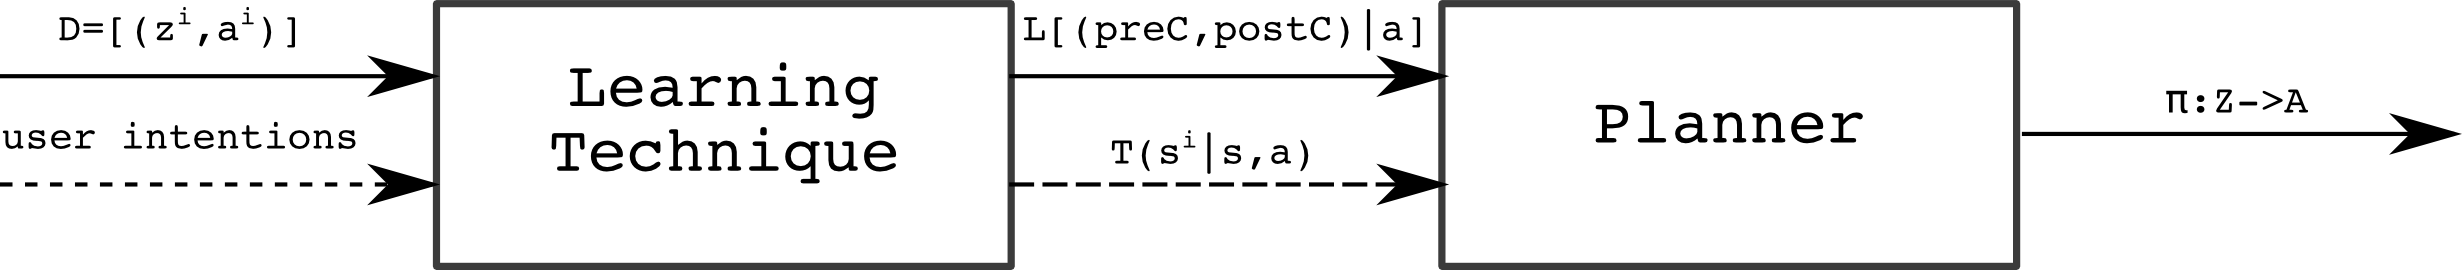
\includegraphics[scale=0.8]{images/plans_policy_derivation.png}
\caption[Deriving a policy : goal based]{Policy Derivation by determining the
goal of the actions \cite{argall_survey_2009}}
\label{goal based learning}
\end{figure}
\subsection {Goal based mapping on relevant features}

The policy learning with the complete set of features of the observed states
faces a drawback that it requires a lot of demonstrations. So to learn on fewer
demonstrations we need to do determine the relevant features of the states and
do the policy learning only based on these relevant features.

When an action shares similar components across multiple demonstrations, it
might suggest that these components are the essential features of the state
that should be reproduced by the robot. In these methods the relevant features
$R$ of the states are determined based on the likelihoods of the
demonstrations, before the goal state prediction.

The policy learning technique first determines which are the relevant aspects
of the states for reproducing the action and these are then provided to the
predictor function which predicts the goal state as illustrated in figure
\ref{feature goal based learning}  (modified from \cite{argall_survey_2009}) .

\begin{figure}[htp]
\centering
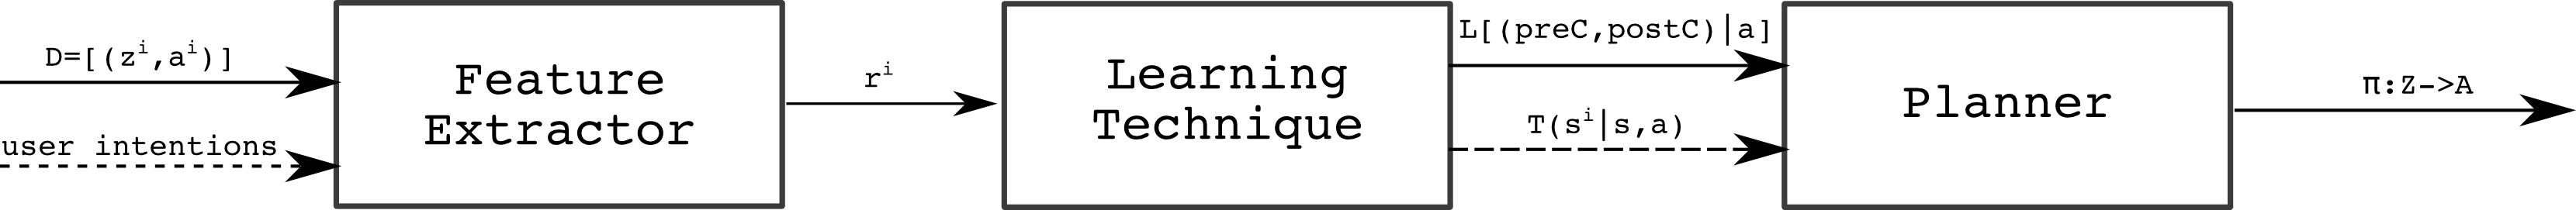
\includegraphics[scale=0.6]{images/features_plans_policy_derivation.png}
\caption[Deriving a policy : feature based ]{Policy derivation using first
extracting relevant features and then determining the goal state of the robot
(modified from \cite{argall_survey_2009})}
\label{feature goal based learning}
\end{figure}

